\documentclass[journal,12pt,twocolumn]{IEEEtran}

\usepackage{setspace}
\usepackage{gensymb}
\singlespacing
\usepackage[cmex10]{amsmath}
\usepackage{multirow}
\usepackage{amsthm}
\usepackage{mathrsfs}
\usepackage{txfonts}
\usepackage{stfloats}
\usepackage{bm}
\usepackage{cite}
\usepackage{cases}
\usepackage{subfig}

\usepackage{longtable}

\usepackage{enumitem}
\usepackage{mathtools}
\usepackage{steinmetz}
\usepackage{tikz}
\usepackage{circuitikz}
\usepackage{verbatim}
\usepackage{tfrupee}
\usepackage[breaklinks=true]{hyperref}
\usepackage{graphicx}
\usepackage{tkz-euclide}

\usetikzlibrary{calc,math}
\usepackage{listings}
    \usepackage{color}                                            %%
    \usepackage{array}                                            %%
    \usepackage{longtable}                                        %%
    \usepackage{calc}                                             %%
    \usepackage{multirow}                                         %%
    \usepackage{hhline}                                           %%
    \usepackage{ifthen}                                           %%
    \usepackage{lscape}     
\usepackage{multicol}
\usepackage{chngcntr}

\DeclareMathOperator*{\Res}{Res}

\renewcommand\thesection{\arabic{section}}
\renewcommand\thesubsection{\thesection.\arabic{subsection}}
\renewcommand\thesubsubsection{\thesubsection.\arabic{subsubsection}}

\renewcommand\thesectiondis{\arabic{section}}
\renewcommand\thesubsectiondis{\thesectiondis.\arabic{subsection}}
\renewcommand\thesubsubsectiondis{\thesubsectiondis.\arabic{subsubsection}}


\hyphenation{op-tical net-works semi-conduc-tor}
\def\inputGnumericTable{}                                 %%

\lstset{
%language=C,
frame=single, 
breaklines=true,
columns=fullflexible
}
\graphicspath{{./Figures/}}
\begin{document}


\newtheorem{theorem}{Theorem}[section]
\newtheorem{problem}{Problem}
\newtheorem{proposition}{Proposition}[section]
\newtheorem{lemma}{Lemma}[section]
\newtheorem{corollary}[theorem]{Corollary}
\newtheorem{example}{Example}[section]
\newtheorem{definition}[problem]{Definition}

\newcommand{\BEQA}{\begin{eqnarray}}
\newcommand{\EEQA}{\end{eqnarray}}
\newcommand{\define}{\stackrel{\triangle}{=}}
\bibliographystyle{IEEEtran}
\raggedbottom
\setlength{\parindent}{0pt}
\providecommand{\mbf}{\mathbf}
\providecommand{\pr}[1]{\ensuremath{\Pr\left(#1\right)}}
\providecommand{\qfunc}[1]{\ensuremath{Q\left(#1\right)}}
\providecommand{\sbrak}[1]{\ensuremath{{}\left[#1\right]}}
\providecommand{\lsbrak}[1]{\ensuremath{{}\left[#1\right.}}
\providecommand{\rsbrak}[1]{\ensuremath{{}\left.#1\right]}}
\providecommand{\brak}[1]{\ensuremath{\left(#1\right)}}
\providecommand{\lbrak}[1]{\ensuremath{\left(#1\right.}}
\providecommand{\rbrak}[1]{\ensuremath{\left.#1\right)}}
\providecommand{\cbrak}[1]{\ensuremath{\left\{#1\right\}}}
\providecommand{\lcbrak}[1]{\ensuremath{\left\{#1\right.}}
\providecommand{\rcbrak}[1]{\ensuremath{\left.#1\right\}}}
\theoremstyle{remark}
\newtheorem{rem}{Remark}
\newcommand{\sgn}{\mathop{\mathrm{sgn}}}
\providecommand{\abs}[1]{\left\vert#1\right\vert}
\providecommand{\res}[1]{\Res\displaylimits_{#1}} 
\providecommand{\norm}[1]{\left\lVert#1\right\rVert}
%\providecommand{\norm}[1]{\lVert#1\rVert}
\providecommand{\mtx}[1]{\mathbf{#1}}
\providecommand{\mean}[1]{E\left[ #1 \right]}
\providecommand{\fourier}{\overset{\mathcal{F}}{ \rightleftharpoons}}
%\providecommand{\hilbert}{\overset{\mathcal{H}}{ \rightleftharpoons}}
\providecommand{\system}{\overset{\mathcal{H}}{ \longleftrightarrow}}
	%\newcommand{\solution}[2]{\textbf{Solution:}{#1}}
\newcommand{\solution}{\noindent \textbf{Solution: }}
\newcommand{\cosec}{\,\text{cosec}\,}
\providecommand{\dec}[2]{\ensuremath{\overset{#1}{\underset{#2}{\gtrless}}}}
\newcommand{\myvec}[1]{\ensuremath{\begin{pmatrix}#1\end{pmatrix}}}
\newcommand{\mydet}[1]{\ensuremath{\begin{vmatrix}#1\end{vmatrix}}}
\newcommand*{\permcomb}[4][0mu]{{{}^{#3}\mkern#1#2_{#4}}}
\newcommand*{\perm}[1][-3mu]{\permcomb[#1]{P}}
\newcommand*{\comb}[1][-1mu]{\permcomb[#1]{C}}
\numberwithin{equation}{subsection}
\makeatletter
\@addtoreset{figure}{problem}
\makeatother
\let\StandardTheFigure\thefigure
\let\vec\mathbf
\renewcommand{\thefigure}{\theproblem}
\def\putbox#1#2#3{\makebox[0in][l]{\makebox[#1][l]{}\raisebox{\baselineskip}[0in][0in]{\raisebox{#2}[0in][0in]{#3}}}}
     \def\rightbox#1{\makebox[0in][r]{#1}}
     \def\centbox#1{\makebox[0in]{#1}}
     \def\topbox#1{\raisebox{-\baselineskip}[0in][0in]{#1}}
     \def\midbox#1{\raisebox{-0.5\baselineskip}[0in][0in]{#1}}
\vspace{3cm}
\title{Assignment 4}
\author{Sujal - AI20BTECH11020}
\maketitle
\newpage
\bigskip
\renewcommand{\thefigure}{\theenumi}
\renewcommand{\thetable}{\theenumi}
Download all python codes from 
\begin{lstlisting}
https://github.com/sujal100/Probability_and_Random_variable/tree/main/exercise_4/codes
\end{lstlisting}

and latex codes from 

\begin{lstlisting}
https://github.com/https://github.com/sujal100/Probability_and_Random_variable/blob/main/exercise_4/exercise_4_main_tex.tex
\end{lstlisting}
\section{Problem [GATE(2012)CS-63]}
An automobile plant contracted to buy shock absorbers from two suppliers $X$ and $Y . X$ supplies $60 \%$ and $Y$ supplies $40 \%$ of the shock absorbers. All shock absorbers are subjected to a quality test. The ones that pass the quality test are considered reliable. Of X's shock absorbers, $96 \%$ are reliable. Of Y's shock absorbers, $72 \%$ are reliable.

The probability that a randomly chosen shock absorber, which is found to be reliable, is made by $Y$ is
(A) 0.288
(B) 0.334
(C) 0.667
(D) 0.720
\section{Solution}
\begin{figure}[htb!]
\begin{center}
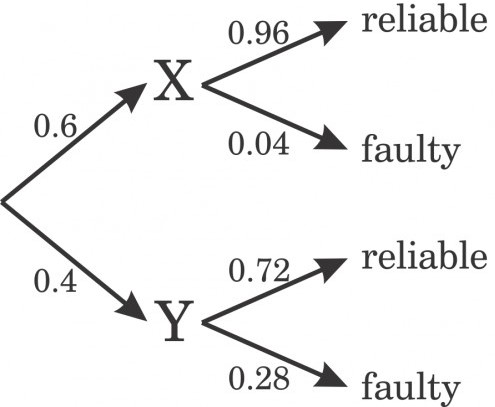
\includegraphics[width=0.5\textwidth]{A_4_1.png}
\end{center}
\end{figure}
Let Consider, Bernoulli random variables say $X,Y$ and $R$.
\begin{table}[h]
\resizebox{\columnwidth}{!}{
\begin{tabular}{|l|l|l|}
\hline
 & Refer to probability that product & Result \\ \hline
$Pr(X=1)$ & from supplier $X$ & $0.6$ \\ \hline
$Pr(Y=1)$ & from supplier $X$ & $0.4$ \\ \hline
$Pr(R=1)$ & is reliable &  \\ \hline
$Pr(R=0)$ & is faulty &  \\ \hline
$Pr(R=1/X=1)$ & from supplier $X$ is reliable & $0.96$ \\ \hline
$Pr(R=1/Y=1)$ & from supplier $Y$ is reliable & $0.72$ \\ \hline
\end{tabular}}
\caption{probability of random variables.}
\label{tab:my-table}
\end{table}
Required probability is $Pr(Y=1|R=1)$.So,
\begin{align}
&Pr(Y=1|R=1)=\frac{Pr(Y=1,R=1)}{Pr(R=1)}\\
&=\frac{Pr(Y=1)Pr(R=1/Y=1)}{Pr(X=1)Pr(R=1/X=1)+Pr(Y=1)P(R=1/Y=1)}\\
&=\frac{(0.4)(0.72)}{(0.6)(0.96)+(0.4)(0.72)}=0.334
\end{align}
\begin{figure}[htb!]
\begin{center}
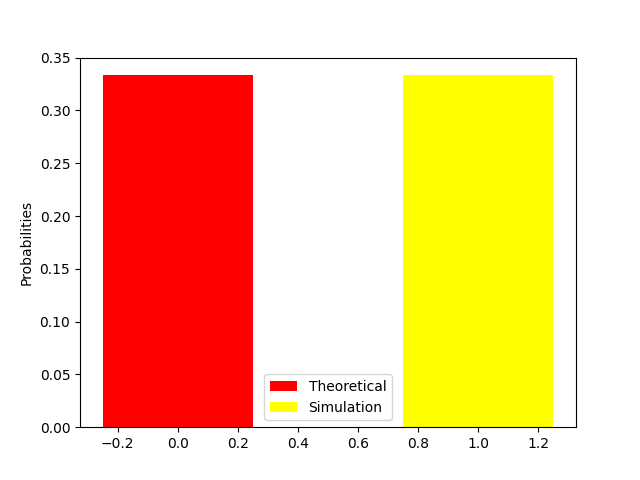
\includegraphics[width=0.6\textwidth]{A_4_2.png}
\caption{Theoretical Vs Simulation}
\end{center}
\end{figure}
Hence $(\mathrm{B})$ is correct option.
\end{document}